\documentclass{article}
\usepackage[section]{placeins}
\usepackage{graphicx}
\usepackage{wrapfig}

\author{Yaghoub Shahmari}
\title{Report - Problem Set no 2}
\date{\today}
\graphicspath{ {../Figs/} }

\begin{document}
    \maketitle
    \section*{Problem 1}
    \textbf{Basic description:}

    We want to simulate the Ballistic Deposition with relaxation.
    So, we will generate some random integers in the surface length range.
    Then, We put The random generated number as the index, and drop the paricle.
    but we have to check the neighbors of the chosen point of the surface.
    If there was a hole in the neighbors, Then the particle will move to that position.
    There is two way to store the data. We can have a 2D Matrix as our deposition layers or have a 1D vector that saves only the height of layers.
    I use the first method for Graphic view and the second to show the $W_{(t)}$ and $H_{(t)}$ in terms of time.

    \textbf{The results:}

    \begin{figure}[!htb]
        \centering
        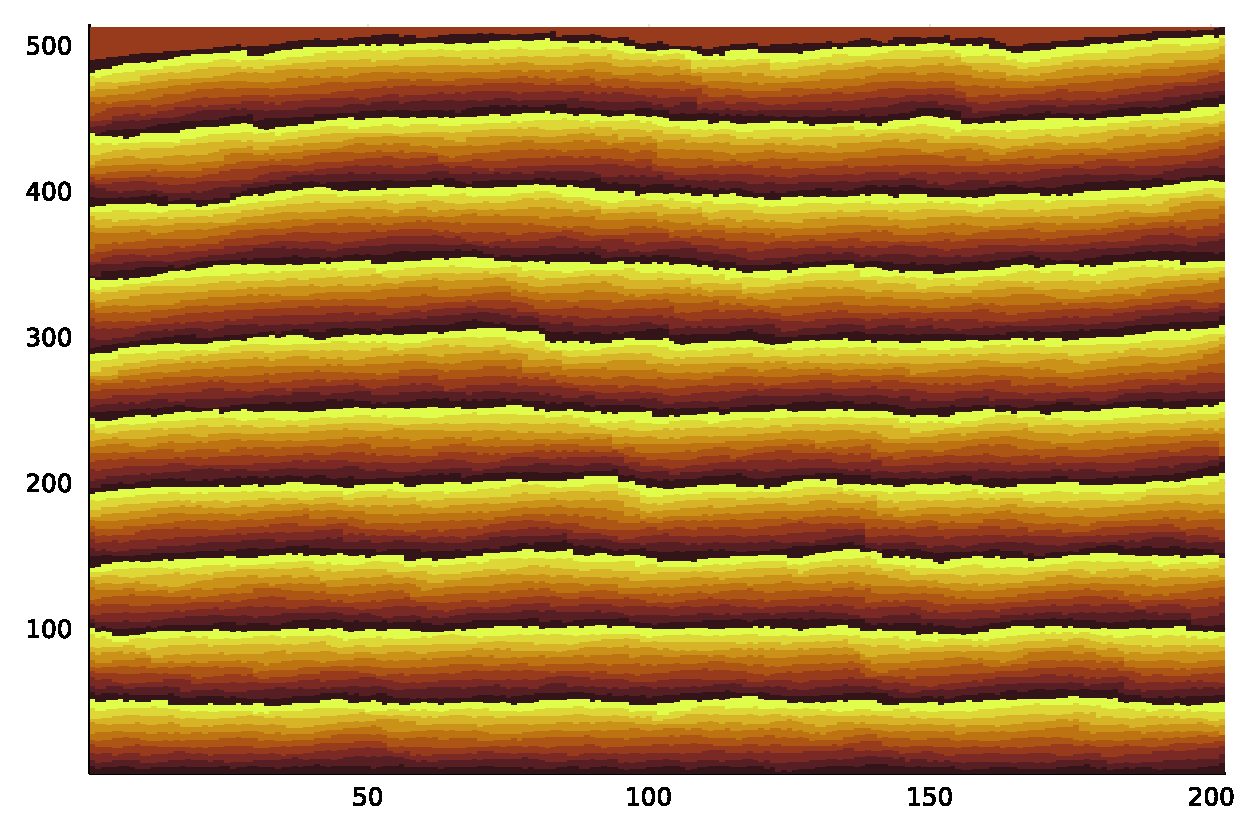
\includegraphics[scale = 0.5]{/Q1/Graphic}
        \label{fig:1.1}
        \caption{Ballistic Deposition with relaxation:
        For one hundred time steps, one thousand particles will drop on a surface of two hundred lengths.
        For every ten steps of time, The color of the visualization will change.}
    \end{figure}

    \pagebreak

    Now we're going to see the statistics of Deposition.
    To have a better view of the dynamic,
    we show our w plot on logarithmic scales.
    For each surface length, we split the time range into exponential periods.
    And for every considered condition, the drop rate of particles is one particle per time unit.

    \begin{figure}[!htb]
        \centering
        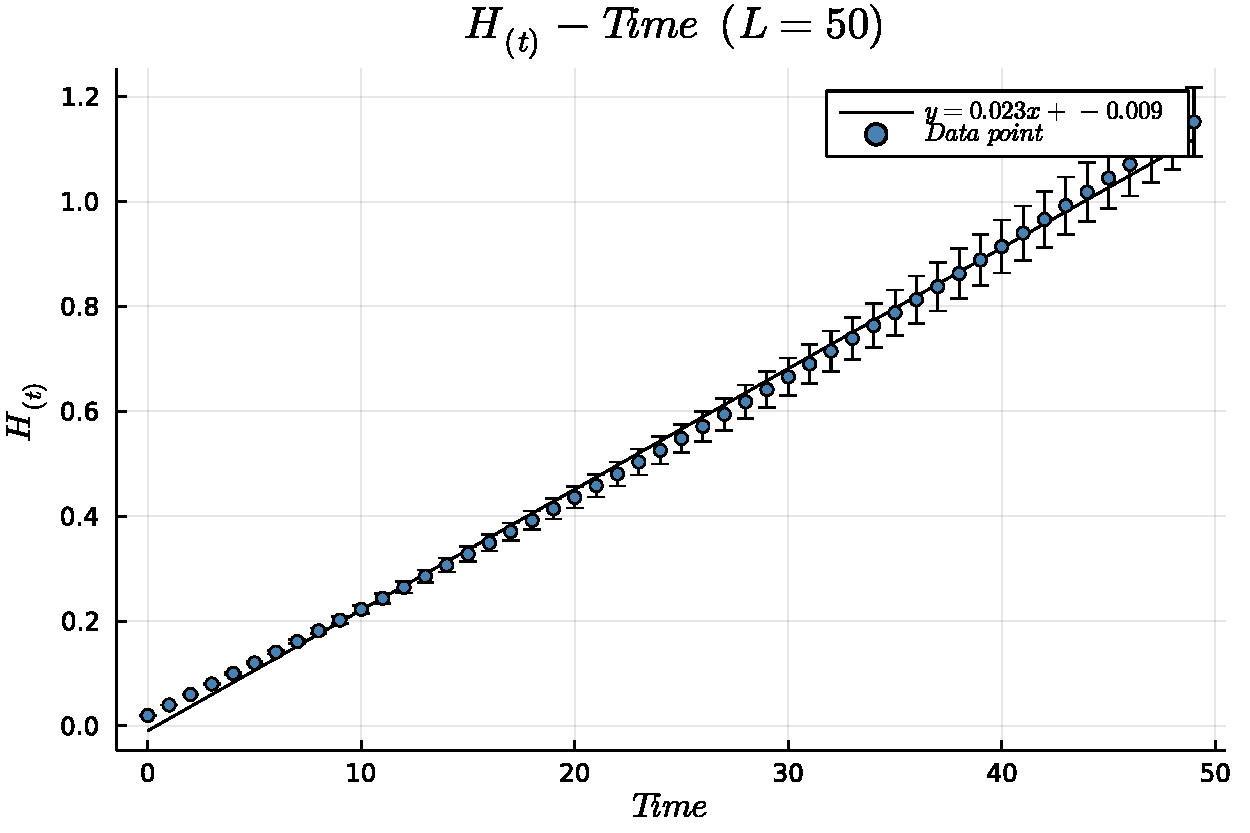
\includegraphics[scale = 0.275]{/Q1/H-t(L=50)}
        \label{fig:1.2}
        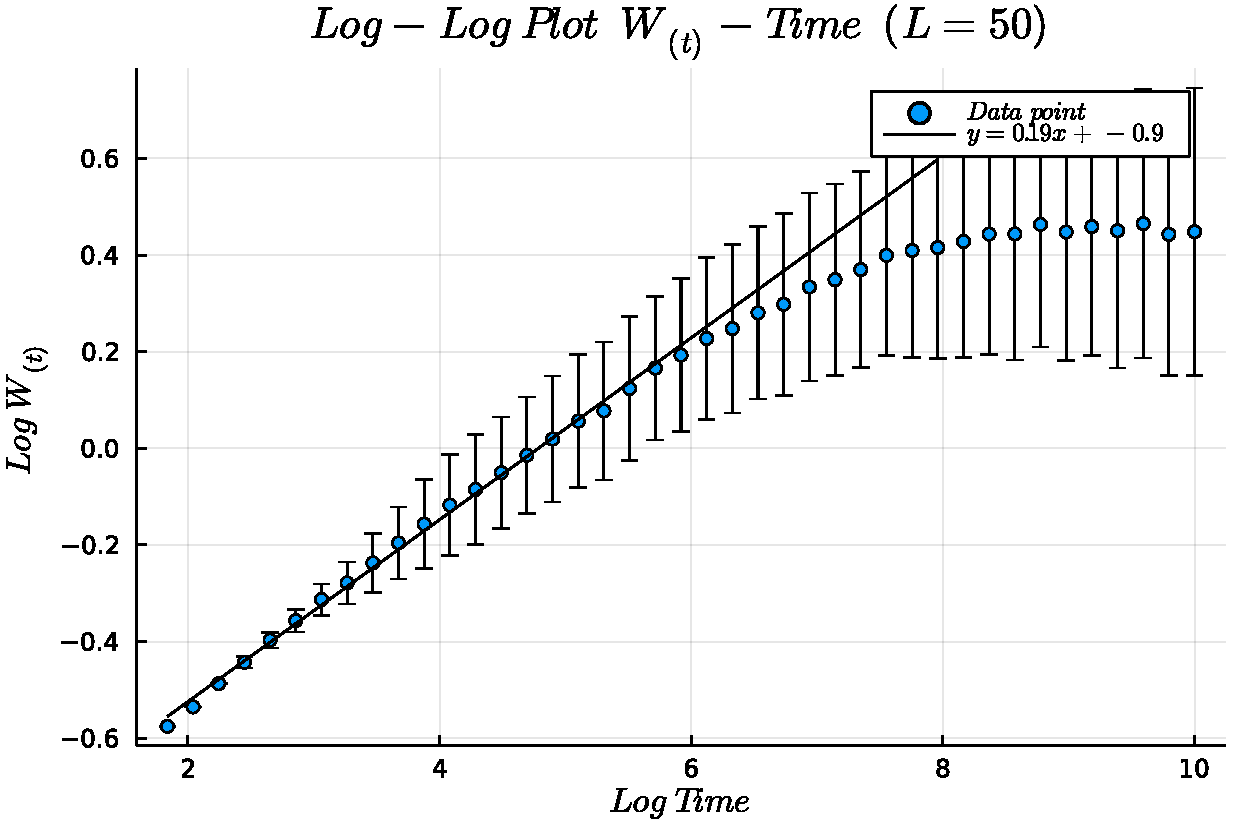
\includegraphics[scale = 0.275]{/Q1/W-t(L=50)}
        \label{fig:1.3}
        \caption{Ballistic Deposition with relaxation for $L=50$}
    \end{figure}
\end{document}